\documentclass[a4,12pt]{scrartcl}

%Basic 
\usepackage[utf8]{inputenc}
\usepackage[ngerman]{babel}
\usepackage[T1]{fontenc}
%Schrift 
\usepackage{textcomp} % Für μ \textmu
%\usepackage{fontspec} 
%\setmainfont{Arial} 
%Zeilenabstand
\usepackage{setspace}
\setstretch {1.3}
\usepackage{float}
\usepackage[bottom = 3.50cm]{geometry}

%Titel Seite
\usepackage{titling} %Wird benötigt damit \maketitle die Variabeln title, author und date nicht überschreibt
\title{Testing}
\subtitle{Projekt: sniffdatel}
\author{David Meister \and Giorgio Vincenti \and Samuel Krieg \and Andreas Stalder}		
 %mit /and können Personen hinzugefügt werden
\date{\today}


%Kopf, Fusszeile
\usepackage{fancyhdr}
\pagestyle{fancy}
\lhead{SW Engineering Projekt FS 2016}
\chead{}
\rhead{sniffdatel}
\lfoot{\thetitle \: v1.0 }
\cfoot{\today }
\rfoot{Seite \thepage}
\renewcommand{\headrulewidth}{0.4pt}

%Bilder
\usepackage{graphicx}

%Zeichnen
\usepackage{tikz}

%Tabellen
\usepackage{booktabs}
\usepackage{longtable}

%Codesnippets
\usepackage{listings}
\lstset{language=java,basicstyle=\footnotesize,frame=single} %backgroundcolor=\color{lightgray}

%Querformat für eine Seite
\usepackage{lscape}
\usepackage{rotating}
\usepackage{pdflscape}

%URL 
\usepackage[colorlinks=true, linkcolor=blue, urlcolor=blue, citecolor=blue]{hyperref}
\urlstyle{same} 


%Loremimpsum
\usepackage{lipsum}



\begin{document}

%\clearpage\maketitle
\begin{titlepage}
	\centering
	\vspace{5cm}
	\begin{center}
	
\includegraphics[width=0.50\textwidth]{logo.png}
	\end{center}
	{\huge\bfseries sniffdatel\par}
	\vspace{8cm}
	\raggedright
	{\bfseries SW Engineering Projekt FS 2016\par}
	{\huge\bfseries Testing\par}
	\vspace{1cm}
	{\theauthor \par}
	{\today\par}

\end{titlepage}

\section{Änderungsgeschichte}

\begin{table}[htb]
\centering
    \begin{tabular}{@{} l l l l@{}}\toprule    
    {Datum} & {Version} & {Änderung} & {Autor}\\ \midrule
    15.05.16 & 1.0 & Erstellung erster Version & Giorgio Vincenti\\ \addlinespace
    26.05.16 & 1.0 & Korrektur & David Meister\\ 
    \bottomrule
    \end{tabular}
\caption{\textbf{Änderungsgeschichte}}
\end{table}
\newpage
%\thispagestyle{empty}
\tableofcontents
\newpage

\section{Einführung}
\subsection{Zweck}
Dieses Dokument dient als Dokumentation für System- und Unittests für das Projekt \textbf{sniffdatel}. 
\subsection{Gültigkeitsbereich}
Das Dokument bezieht sich auf die Software \textbf{sniffdatel}, welche im Rahmen des Moduls Engineeringprojekt des Frühjahrssemester 2016 entwickelt wird und ist während des gesamten Projekts gültig. 
\subsection{Referenzen}
\begin{itemize}
\item doc/02\_projektplan/Projektplan\_v1.7
\item doc/03\_analyse/Anforderungsspezifikationen\_v1.1
\item doc/03\_analyse/Domainanalyse\_v1.1
\item doc/04\_design/Architektur\_v1.1
\item doc/04\_design/ExternesDesign\_v1.0
\item doc/05\_qm/Qualitätsmassnahmen\_v1.1
\item doc/07\_tests/UsabilityTests\_v1.0
\end{itemize}

\noindent Diese Dokumente sind bei uns auf der Dropbox oder auf Github zu finden. Für den Betreuer sind die Dokumente auf Redmine vorhanden. 
\newpage

\section{Systemtest}

\subsection{UC1: select interfaces}
\begin{table}[H]
\centering
    \begin{tabular}{@{} p{0.5cm} p{7cm} p{6cm} @{}}\toprule    
    {Nr} & {Beschreibung} & {Erwartetes Ergebnis}\\ \midrule
    1 & Der Benutzer klickt auf den Interface Button im GUI. & Programm liefert Interfaceauswahl in neuem Fenster.\\ \addlinespace
    2 & Der Benutzer wählt ein Interface aus der Liste aus und bestätigt seine Auswahl mit START. & Interface Fenster verschwindet, Scanvorgang von Programm startet automatisch. \\
    \bottomrule
    \end{tabular}
\caption{\textbf{UC1}}
\end{table}

\subsubsection{Voraussetzungen}
Die Applikation ist gestartet und das Gerät ist mit einer beliebigen Schnittstelle mit dem Netzwerk verbunden. 

\subsubsection{Testergebnisse}
\begin{table}[H]
\centering
    \begin{tabular}{@{} p{0.5cm} p{11cm} p{2cm} @{}}\toprule    
    {Nr} & {Beschreibung} & {Ergebnis}\\ \midrule
    1 & Das Programm liefert dem Benutzer eine Liste mit allen möglichen Interfaces. & OK\\ \addlinespace
   	2 & Scanvorgang von Programm wurde automatisch gestartet. & OK\\
    \bottomrule
    \end{tabular}
\caption{\textbf{Ergebnisse}}
\end{table}

\newpage

\subsection{UC2: collecting sessions}
\begin{table}[H]
\centering
    \begin{tabular}{@{} p{0.5cm} p{7cm} p{6cm} @{}}\toprule    
    {Nr} & {Beschreibung} & {Erwartetes Ergebnis}\\ \midrule
    1 & Der Benutzer wartet auf eingehende Sessions & Programm listet während Scanfunktion alle VoIP Sessions auf, welche ab den Zeitpunkt des Scanvorgang aufgebaut werden.\\ \addlinespace
    2 & Neue Sessions werden im Programm angezeigt & Eine gefundene Session hat verschiedene SIP Status, die sich je nach Verbindungsstatus verrändern (Ringing,Active Call, Ack, Bye). Session Details (Session Name, IP und MAC Adressen der Teilnehmer und Codec) werden angezeigt\\ \addlinespace
    3 & Anzeigen beendeter VoIP Sessions. & VoIP Anrufen die beendet wurden, fallen nicht aus Liste. Der SIP Status ändert sich in BYE.\\ \addlinespace
    4 & Benutzer klickt STOP CAPTURING SESSIONS. & Programm hört auf zu scannen, neue VoIP Sessions werden weder detektiert noch angezeigt\\ \addlinespace
    5 & Benutzer klickt RESTART CURRENT CAPTURE & Capture wird neu gestartet, aktuelle Sessions verschwinden, bei neuen eingehenden Sessions werden diese wieder angezeigt\\    
    \bottomrule
    \end{tabular}
\caption{\textbf{UC2}}
\end{table}

\subsubsection{Voraussetzungen}
Aktionen gemäss UC1 wurden durchgeführt. VoIP Verkehr ist auf dem dort ausgewählten Interface tatsächlich vorhanden.

\subsubsection{Testergebnisse}
\begin{table}[H]
\centering
    \begin{tabular}{@{} p{0.5cm} p{11cm} p{2cm} @{}}\toprule    
    {Nr} & {Beschreibung} & {Ergebnis}\\ \midrule
    1 & Programm listet während Scanfunktion alle VoIP Sessions auf, welche ab den Zeitpunkt des Scanvorgang aufgebaut werden. & OK\\ \addlinespace
   	2 & Eine gefundene Session hat verschiedene SIP Status, die sich je nach Verbindungsstatus verrändern (Ringing,Active Call, Ack, Bye). Session Details (Session Name, IP und MAC Adressen der Teilnehmer und Codec) werden angezeig) & OK\\ \addlinespace
    3 & VoIP Anrufen die beendet wurden, fallen nicht aus Liste. Der SIP Status ändert sich in BYE. & OK\\ \addlinespace
    4 & Programm hört auf zu scannen, neue VoIP Sessions werden weder detektiert noch angezeigt & OK\\ \addlinespace
    5 & Capture wird neu gestartet, aktuelle Sessions verschwinden, bei neuen eingehenden Sessions werden diese wieder angezeigt & OK\\
    \bottomrule
    \end{tabular}
\caption{\textbf{Ergebnisse}}
\end{table}
\newpage

\subsection{UC3: listening conversations}
\begin{table}[H]
\centering
    \begin{tabular}{@{} p{0.5cm} p{7cm} p{6cm} @{}}\toprule    
    {Nr} & {Beschreibung} & {Erwartetes Ergebnis}\\ \midrule
    1 & Der Benutzer will auf den Play Button drücken bei Sessions die kein ACTIVE CALL Status haben. & Der Play Button kann nicht gedrückt werden. \\ \addlinespace
    2 & Play Button erscheint & Wenn eine aktive Session (Session Status Active Call)angeklickt wird kann der Play Button gedrückt werden\\ \addlinespace
    3 & Stopbutton erscheint & Wenn ein aktives Gespräch abgespielt wird, kann die Audiowiedergabe mittels Stop Button abgebrochen werden\\ \addlinespace
    4 & Wiedergabe fortführen & Wenn eine Wiedergabe gestoppt wurde, kann diese erneut mittels Playbutton fortgeführt werden\\ \addlinespace
    5 & Abbruch durch Scan restart & Wenn bei einer laufenden Wiedergabe der Button restart current capture gedrückt wird, soll die Audiowiedergabe abgebrochen werden und ein neuer Scan soll gestartet werden\\ \addlinespace
    6 & Gesprächsrichtung & Im Dropdown kann die Gesprächsrichtung (Left -> Right, Right -> Left, Both) festgelegt werden. Nachdem der Play Button gedrückt wurde wird gemäss Auswahl abgespielt\\
    \bottomrule
    \end{tabular}
\caption{\textbf{UC3}}
\end{table}

\subsubsection{Voraussetzungen}
Mindestens eine aktive VoIP Session wird gescannt. Der verwendete Codec muss von sniffdatel unterstützt werden.

\subsubsection{Testergebnisse}
\begin{table}[H]
\centering
    \begin{tabular}{@{} p{0.5cm} p{11cm} p{2cm} @{}}\toprule    
    {Nr} & {Beschreibung} & {Ergebnis}\\ \midrule
    1 & Der Play Button kann nicht gedrückt werden. & OK\\ \addlinespace
   	2 & Wenn eine aktive Session (Session Status Active Call)angeklickt wird kann der Play Button gedrückt werden & OK\\ \addlinespace
   	3 & Wenn ein aktives Gespräch abgespielt wird, kann die Audiowiedergabe mittels Stop Button abgebrochen werden & OK\\ \addlinespace
   	4 & Wenn eine Wiedergabe gestoppt wurde, kann diese erneut mittels Playbutton fortgeführt werden & OK\\ \addlinespace
    5 & Wenn bei einer laufenden Wiedergabe der Button restart current capture gedrückt wird, soll die Audiowiedergabe abgebrochen werden und ein neuer Scan soll gestartet werden & FAIL\\ \addlinespace
    6 & Im Dropdown kann die Gesprächsrichtung (Left -> Right, Right -> Left, Both) festgelegt werden. Nachdem der Play Button gedrückt wurde wird gemäss Auswahl abgespielt & OK\\    
    \bottomrule
    \end{tabular}
\caption{\textbf{Ergebnisse}}
\end{table}
\newpage

\section{Unit Test}
Für alle wichtigen Klassen wurden Unit Tests geschrieben. Als Test-library haben wir JUnit4 eingesetzt. In diesem Kapitel beschreiben wir die jeweils erstellten Tests.  
\subsection{Verwendete Tools}
Alle verwendete Tools funktionieren mit der Eclipse Entwicklungsumgebung. 
\subsubsection{JUnit4}
JUnit ist ein Testframework mit welchem man Unit Test schreiben kann. Es kann als Library ins Projekt eingebunden werden. Wir verwenden die Version 4.
\begin{itemize}
\item Homepage: junit.org/junit4/
\end{itemize}
\subsubsection{EclEmma}
EclEmma ist ein gratis Tool und wird verwendet um die Testabdeckung anzuzeigen. 
\begin{itemize}
\item Homepage: eclemma.org
\end{itemize}
\subsubsection{Mockito}
Mockito ist ein mocking framework für Unit Tests in Java. Library muss heruntergeladen und ins Projekt eingebunden werden. 
\begin{itemize}
\item Homepage: mockito.org
\end{itemize}
\newpage

\subsection{Erwartete Testabdeckung}
Durch die Tests wollen wir eine möglichst hohe Abdeckung(90\%) des nicht trivialen Codes.

\subsubsection{Ausgeschlossene Packages und Klassen}
\begin{itemize}
\item \textbf{ch.sniffdatel.basis.processedData}
\begin{itemize}
\item Session.java
\item SessionParticipant.java
\item SipSdpObserver.java
\end{itemize}
\item \textbf{ch.sniffdatel.basis.rawDataType}
\begin{itemize}
\item RtpPacket.java
\item SdpPacket.java
\item SipPacket.java
\end{itemize}
\item \textbf{ch.sniffdatel.presentation}
\begin{itemize}
\item Main.java
\end{itemize}
\item \textbf{ch.sniffdatel.presentation.model} 
\begin{itemize}
\item Interface.java
\item SessionModel.java
\end{itemize}
\item \textbf{ch.sniffdatel.presentation.view}
\begin{itemize}
\item InterfaceSelectionController.java
\item SessionOverviewController.java
\end{itemize}
\item \textbf{ch.sniffdatel.service.packetParser}
\begin{itemize}
\item Interfaces.java
\end{itemize}
\end{itemize}
Die gesamte GUI Implementation mit dem Java FX Framework, private Methoden und die DTOs aus dem basis.rawDataType Package werden nicht getestet, sowie sämtliche getter- und setter Methoden. Es entfallen somit viele Klassen für Unit Tests. 
\newpage

\subsection{Testklassen Übersicht}
\begin{figure} [H]
	\begin{center}
	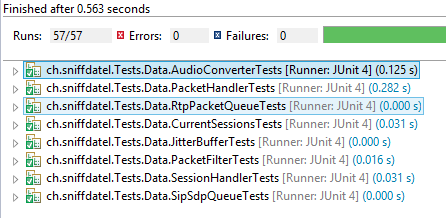
\includegraphics[width=0.50\textwidth]{./pictures/TestsComplete.png}
	\label{Bild Referenz}
	\end{center}
\end{figure}
\textbf{Initialisierung der Objekte bei allen Testklassen}
\begin{table}[H]
\centering
    \begin{tabular}{@{} p{3.5cm} p{10cm} @{}}\toprule    
    {Testname} & {Beschreibung}\\ \midrule
    setUp() & @Before: Initialisiert alle notwendigen Feldern\\ \addlinespace
   	tearDown() & @After: Resetet alle notwendigen Feldern\\ \addlinespace
   	@Mock & Definition der Mock Objekte zu Beginn der Testklasse \\
    \bottomrule
    \end{tabular}
\caption{\textbf{Allgemeine Methoden in Testklassen}}
\end{table}
\newpage

\subsubsection{Testklasse: RtpPacketQueueTests}
\begin{figure} [H]
	\begin{center}
	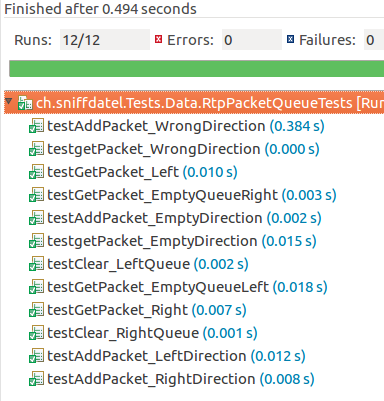
\includegraphics[width=0.60\textwidth]{./pictures/RtpPacketQueueTests.png}
	\label{Bild Referenz}
	\end{center}
\end{figure}
\textbf{Beschreibung der einzelnen Tests}
\begin{longtable}{ p{7cm} p{7cm} }  
   {Testname} & {Beschreibung}\\ \midrule
    testAddPacket\_LeftDirection() & Testet das hinzufügen eines Pakets in die Linke Queue, mit der Richtung Links.\\ \addlinespace
    testAddPacket\_RightDirection() & Testet das hinzufügen eines Packets in die Rechte Queue, mit der Richtung Rechts. \\ \addlinespace
    testAddPacket\_WrongDirection() & Testet ob eine Exception geworfen wird, falls das Paket eine falsche Richtung enthält.\\ \addlinespace
    testAddPacket\_EmptyDirection() & Testet ob eine Exception geworfen wird, falls das Paket über keine Richtung verfügt. \\ \addlinespace
    testGetPacket\_Left() & Testst ob das richtige Paket zurückgegeben wird, mit der angabe der Richtung Links. \\ \addlinespace
    testGetPacket\_Right() & Testst ob das richtige Paket zurückgegeben wird, mit der angabe der Richtung Rechts. \\ \addlinespace
    testGetPacket\_WrongDirection() & Testet ob eine Exception geworfen wird, falls die Richtung nicht Links oder Rechts ist. \\ \addlinespace
    testGetPacket\_EmptyQueueRight() & Testet ob eine Exception geworfen wird, falls die Richtung leer ist. \\ \addlinespace
    testGetPacket\_EmptyQueueLeft() & Testet ob eine Exception geworfen wird, falls die Linke Queue leer ist. \\ \addlinespace
    testGetPacket\_EmptyDirection() & Testet ob eine Exception geworfen wird, falls die Rechte Queue leer ist.\\ \addlinespace
    testClear\_RightQueue() & Testet die Funktion clear() auf die Rechte Queue. \\ \addlinespace
    testClear\_LeftQueue() & Testet die Funktion clear() auf die Linke Queue.\\
\caption{\textbf{RtpPacketQueueTests: Testmethoden}}
\end{longtable}

\noindent \textbf{Mock-Objekte:} RtpPacket.class\\
\textbf{EclEmma-Abdeckung:} 100\%

\subsubsection{Testklasse: SipSdpQueueTests}
\begin{figure} [H]
	\begin{center}
	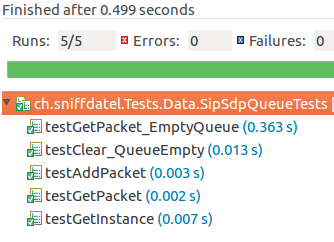
\includegraphics[width=0.60\textwidth]{./pictures/SipSdpQueueTests.png}
	\label{Bild Referenz}
	\end{center}
\end{figure}

\textbf{Beschreibung der einzelnen Tests}
\begin{longtable}{ p{7cm} p{7cm} }  
    {Testname} & {Beschreibung}\\ \midrule
    testAddPacket() & Testet das hinzufügen eines Pakets in die Queue.\\ \addlinespace
    testGetPacket() & Testet ob das richtige Paket zurückgegeben wird.\\ \addlinespace
    testGetInstance() & Testet ob die erstellte Instanz der richtige Typ hat.\\ \addlinespace
    testClear\_EmptyQueue() &  Testet ob Null ausgegeben wird, falls die Queue leer ist.\\ \addlinespace
    testGetPacket\_QueueEmpty() & Testet ob Null ausgegeben wird, falls die Methode getPacket() auf eine leere Queue ausgeführt wird. \\
\caption{\textbf{SipSdpQueueTests: Testmethoden}}
\end{longtable}

\noindent \textbf{Mock-Objekte:} SipPacket.class \\
\textbf{EclEmma-Abdeckung:} 100\%

\subsubsection{Testklasse: JitterBufferTests}
\begin{figure} [H]
	\begin{center}
	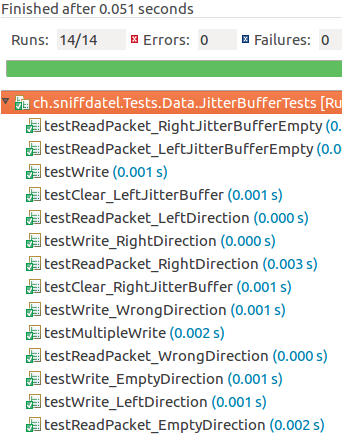
\includegraphics[width=0.60\textwidth]{./pictures/JitterBufferTests.png}
	\label{Bild Referenz}
	\end{center}
\end{figure}

\textbf{Beschreibung der einzelnen Tests}
\begin{longtable}{ p{7cm} p{7cm} }   
    {Testname} & {Beschreibung}\\ \midrule
    testReadPacket\_RightJitterBufferEmpty() & Testst ob die Methode Null zurück gibt, falls auf einer leeren Queue gelesen wird, in Richtung Rechts. \\ \addlinespace
    testReadPacket\_LeftJitterBufferEmpty() & Testst ob die Methode Null zurück gibt, falls auf einer leeren Queue gelesen wird, in Richtung Links. \\ \addlinespace
    testReadPacket\_LeftDirection() & Testet ob das richtige Paket gelesen wird, in der linken Queue.\\ \addlinespace
    testReadPacket\_RightDirection() & Testet ob das richtige Paket gelesen wird, in der rechten Queue.  \\ \addlinespace
    testReadPacket_\WrongDirection() & Testet ob eine Exception geworfen wird falls die Richtung nicht links oder rechts ist. \\ \addlinespace
    testReadPacket_\EmptyDirection() & Testet ob eine Exception geworfen wird falls die Richtung leer ist. \\ \addlinespace
    testWrite() & Testet ob ein einzelnes Paket in die Queue geschrieben wird.\\ \addlinespace
    testWrite\_LeftDirection() &  Testst ob ein einzelnes Paket in die Linke Queue geschrieben wird.\\ \addlinespace
    testWrite\_RightDirection() & Testet ob ein einzelnes Paket in die Rechte Queue geschrieben wird. \\ \addlinespace
    testMultipleWrite() & Testet ob mehrere Pakete in die Queue geschrieben werden können.\\ \addlinespace
    testWrite\_WrongDirection() &  Testet ob eine Exception geworfen wird, falls eine falsche Richtung angegeben wird. \\ \addlinespace
    testWrite\_EmptyDirection() & Testet ob eine Exception geworfen wird, falls eine leere Richtung angegeben wird.\\ \addlinespace
    testClear\_LeftJitterBuffer() &  Testet ob die Funktion clear() auf die Linke Queue angewendet wird.\\ \addlinespace
    testClear\_RightJitterBuffer() & Testet ob die Funtion clear() auf die Rechte Queue angewendet wird.  \\ 
\caption{\textbf{JitterBufferTests: Testmethoden}}
\end{longtable}

\noindent \textbf{Mock-Objekte:} keine vorhanden.\\
\textbf{EclEmma-Abdeckung:} 94.9\%

\subsubsection{Testklasse: PacketHandlerTests}
\begin{figure} [H]
	\begin{center}
	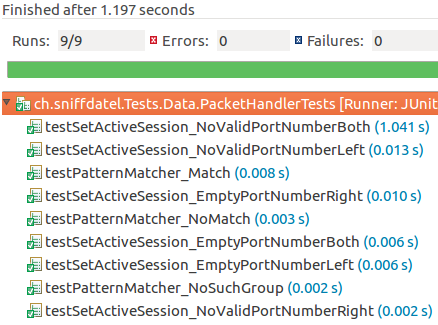
\includegraphics[width=0.60\textwidth]{./pictures/PacketHandlerTests.png}
	\label{Bild Referenz}
	\end{center}
\end{figure}

\textbf{Beschreibung der einzelnen Tests}
\begin{longtable}{ p{9cm} p{6.5cm} }    
    {Testname} & {Beschreibung}\\ \midrule
    testSetActiveSession\_NoValidPortNumberBoth() & Testet ob bei zwei falschen Portnummern eine Exception geworfen wird\\ \addlinespace
    testSetActiveSession\_NoValidPortNumberLeft() & Testet ob bei einer falschen Portnummer eine Exception geworfen wird\\ \addlinespace
    testSetActiveSession\_NoValidPortNumberRight() & Testet ob bei einer falschen Portnummer eine Exception geworfen wird\\ \addlinespace
    testSetActiveSession\_EmptyPortNumberRight() & Testet ob bei einer leeren Portnummer eine Exception geworfen wird\\ \addlinespace
    testSetActiveSession\_EmptyPortNumberLeft() & Testet ob bei einer leeren Portnummer eine Exception geworfen wird\\ \addlinespace
    testSetActiveSession\_EmptyPortNumberBoth() & Testet ob bei zwei leeren Portnummern eine Exception geworfen wird\\ \addlinespace
  	testPatternMatcher\_Match() & Testet ob bei einem Match der erwartete String zurückgegeben wird\\ \addlinespace
    testPatternMatcher\_NoMatch() & Testet das Verhalten wenn der Regex nichts matched\\ \addlinespace
    testPatternMatcher\_NoSuchGroup() & Testet das Verhalten bei falscher Matchergruppe\\ 
\caption{\textbf{PacketHandlerTests: Testmethoden}}
\end{longtable}

\noindent \textbf{Mock-Objekte:} PcapPacket.class\\
\textbf{EclEmma-Abdeckung:} 21.5\%


\subsubsection{Testklasse: PacketFilterTests}
\begin{figure} [H]
	\begin{center}
	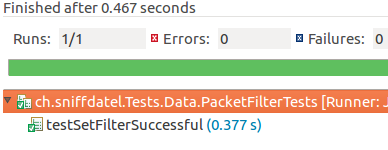
\includegraphics[width=0.60\textwidth]{./pictures/PacketFilterTests.png}
	\label{Bild Referenz}
	\end{center}
\end{figure}

\textbf{Beschreibung der einzelnen Tests}
\begin{longtable}{ p{7cm} p{7cm} }     
    {Testname} & {Beschreibung}\\ \midrule
    testSetFilterSuccessful() & Testst ob der korrekte Filter angewendet wurde und gibt das pcap Objekt in diesem Fall zurück.\\ 
\caption{\textbf{PacketFilterTests: Testmethoden}}
\end{longtable}

\noindent \textbf{Mock-Objekte:} Pcap.class\\
\textbf{EclEmma-Abdeckung:} 65.7\%

\subsubsection{Testklasse: CurrentSessionsTests}
\begin{figure} [H]
	\begin{center}
	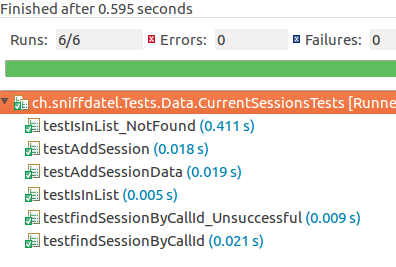
\includegraphics[width=0.60\textwidth]{./pictures/CurrentSessionTests.png}
	\label{Bild Referenz}
	\end{center}
\end{figure}

\textbf{Beschreibung der einzelnen Tests}
\begin{longtable}{ p{7cm} p{7cm} }   
    {Testname} & {Beschreibung}\\ \midrule
    testAddSession() & Testet ob man einzelne Sessions hinzufügen kann.\\ \addlinespace
    testAddSessionData() & Testet ob man die Sessions die zuvor in die ArrayList hinzugefügt wurden, in die ObservableList hinzugefügt werden können.  \\ \addlinespace
    testIsInList() & Testet ob man Sessions in der ObservableList finden kann, anhand eines Session Name.\\ \addlinespace
    testIsInList\_NotFound() & Testet ob das Programm eine -1 zurückgibt falls der Session Name nicht in der ObservableList gefunden wurde. \\ \addlinespace
    testFindSessionByCallId() & Testet ob man Sessions anhand einer ID in der ArrayList finden kann.\\ \addlinespace
    testFindSessionByCallId\_Unsuccessful() & Testet ob das Programm Null zurückgibt falls die Session, in der ArrayList, anhand der Id nicht gefunden werden konnte. \\
\caption{\textbf{CurrentSessionsTests: Testmethoden}}
\end{longtable}

\noindent \textbf{Mock-Objekte:} Session.class und SessionParticipant.class\\
\textbf{EclEmma-Abdeckung:} 85\%

\subsubsection{Testklasse: AudioConveterTests}
\begin{figure} [H]
	\begin{center}
	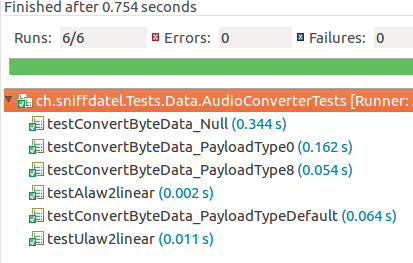
\includegraphics[width=0.60\textwidth]{./pictures/AudioConverterTests.png}
	\label{Bild Referenz}
	\end{center}
\end{figure}

\textbf{Beschreibung der einzelnen Tests}
\begin{longtable}{ p{9cm} p{6.45cm} }   
    {Testname} & {Beschreibung}\\ \midrule
    testConvertByteData\_PayloadType0() & Testet ob beim Payload Type 0 (ulaw) ein bestimmtes Byte Array zurückgegeben wird\\ \addlinespace
    testConvertByteData\_PayloadType8() & Testet ob beim Payload Type 8 (alaw) ein bestimmtes Byte Array zurückgegeben wird\\ \addlinespace
    testConvertByteData\_PayloadTypeDefault() & Testet das Verhalten bei einem anderen Payload Type\\ \addlinespace
    testConvertByteData\_Null() & Testet ob bei einem leeren Array eine Exception geworfen wird\\ \addlinespace
    testAlaw2linear() & Testet die Konvertierung\\ \addlinespace
    testUlaw2linear() & Testet die Konvertierung\\
\caption{\textbf{AudioConverterTests: Testmethoden}}
\end{longtable}

\noindent \textbf{Mock-Objekte:} RtpPacket.class\\
\textbf{EclEmma-Abdeckung:} 80.6\%

\subsubsection{Testklasse: SessionHandlerTests}
\begin{figure} [H]
	\begin{center}
	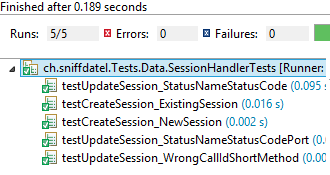
\includegraphics[width=0.60\textwidth]{./pictures/SessionHandlerTests.png}
	\label{Bild Referenz}
	\end{center}
\end{figure}

\textbf{Beschreibung der einzelnen Tests}
\begin{longtable}{ p{9cm} p{6.5cm} }     
    {Testname} & {Beschreibung}\\ \midrule
    testCreateSession\_ExistingSession() & Testet, dass keine Session hinzugefügt wird, sofern sie bereits erstellt wurde\\ \addlinespace
    testCreateSession\_NewSession() & Testet, dass die Session hinzugefügt wird, sofern sie noch nicht erstellt wurde\\ \addlinespace
    testUpdateSession\_StatusNameStatusCode() & Testet, ob die Parameter der Session nach Aufruf der Update Methode geändert wurden\\ \addlinespace
    testUpdateSession\_WrongCallIdShortMethod() & Testet, dass bei einer falschen Eingabe der Call ID nichts geändert wird\\ \addlinespace
    testUpdateSession\_StatusNameStatusCodePort() & Testet, ob die Parameter der Session nach Aufruf der Update Methode geändert wurden\\
\caption{\textbf{SessionHandlerTests: Testmethoden}}
\end{longtable}

\noindent \textbf{Mock-Objekte:} SipPacket.class, SipSdpQueue .class, SdpPacket .class\\
\textbf{EclEmma-Abdeckung:} 56.2\%

\subsection{Definitive Testabdeckung}
Nachdem wir alle Unit Tests zu unseren Klassen geschrieben haben, müssen wir prüfen ob die Erwartungen von 90\% Abdeckung erfüllt wurden. Dies wird anhand des Tools EclEmma im Eclipse durchgeführt. Insgesamt haben wir 57 Tests für unsere Klassen geschrieben. Hier einen Screenshot der Abdeckung gemäss EclEmma: 
\begin{figure} [H]
	\begin{center}
	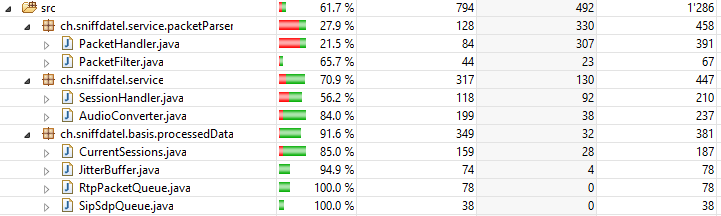
\includegraphics[width=0.80\textwidth]{./pictures/TotalCoverage.png}
	\label{Bild Referenz}
	\end{center}
\end{figure}

\subsubsection{Bemerkung} 
Unsere testbaren Klassen erreichen eine Coverage von gerade einmal 61.7\%. Somit haben wir unser Ziel von 90\% Coverage deutlich verfehlt. Die Klassen PacketHandler, PacketFilter und SessionHandler haben teils grosse Methoden, welche mit Objekten von Frameworks wie jnet Pcap oder JavaFX arbeiten. Solche Objekte sind extrem schwierig zu Mocken und somit ist ein isolierter Unit Test fast nicht möglich. Es müssten aufwändige Refactorings durchgeführt werden, um solche Methoden für uns testbar zu machen.
\newpage

\section{Usability Tests}
Das Kapitel Usability Tests wird in einem seperaten Dokument behandelt. 
\begin{itemize}
\item doc/07\_tests/UsabilityTests\_v1.0
\end{itemize}
\end{document}
